%%%%%%%%%%%%%%%%%%%%%%%%%%%%%%%%%%%%%%%%%
% Structured General Purpose Assignment
% LaTeX Template
%
% This template has been downloaded from:
% http://www.latextemplates.com
%
% Original author:
% Ted Pavlic (http://www.tedpavlic.com)
%
% Note:
% The \lipsum[#] commands throughout this template generate dummy text
% to fill the template out. These commands should all be removed when 
% writing assignment content.
%
%%%%%%%%%%%%%%%%%%%%%%%%%%%%%%%%%%%%%%%%%

%----------------------------------------------------------------------------------------
%	PACKAGES AND OTHER DOCUMENT CONFIGURATIONS
%----------------------------------------------------------------------------------------

\documentclass{article}

\usepackage{fancyhdr} % Required for custom headers
\usepackage{lastpage} % Required to determine the last page for the footer
\usepackage{extramarks} % Required for headers and footers
\usepackage{graphicx} % Required to insert images
\usepackage{lipsum} % Used for inserting dummy 'Lorem ipsum' text into the template
\usepackage{mathtools, bm}
\usepackage{amssymb, bm}
\usepackage{graphicx}
\usepackage{algorithmic}

% Margins
\topmargin=-0.45in
\evensidemargin=0in
\oddsidemargin=0in
\textwidth=6.5in
\textheight=9.0in
\headsep=0.25in 

\linespread{1.1} % Line spacing

% Set up the header and footer
\pagestyle{fancy}
\lhead{\hmwkAuthorName} % Top left header
\chead{\hmwkClass\ (\hmwkClassInstructor\ \hmwkClassTime): \hmwkTitle} % Top center header
\rhead{\firstxmark} % Top right header
\lfoot{\lastxmark} % Bottom left footer
\cfoot{} % Bottom center footer
\rfoot{Page\ \thepage\ of\ \pageref{LastPage}} % Bottom right footer
\renewcommand\headrulewidth{0.4pt} % Size of the header rule
\renewcommand\footrulewidth{0.4pt} % Size of the footer rule

\setlength\parindent{0pt} % Removes all indentation from paragraphs

%----------------------------------------------------------------------------------------
%	DOCUMENT STRUCTURE COMMANDS
%	Skip this unless you know what you're doing
%----------------------------------------------------------------------------------------

% Header and footer for when a page split occurs within a problem environment


% Header and footer for when a page split occurs between problem environments


\setcounter{secnumdepth}{0} % Removes default section numbers
\newcounter{homeworkProblemCounter} % Creates a counter to keep track of the number of problems

\newcommand{\homeworkProblemName}{}
\newenvironment{homeworkProblem}[1][Problem \arabic{homeworkProblemCounter}]{ % Makes a new environment called homeworkProblem which takes 1 argument (custom name) but the default is "Problem #"
\stepcounter{homeworkProblemCounter} % Increase counter for number of problems
\renewcommand{\homeworkProblemName}{#1} % Assign \homeworkProblemName the name of the problem
\section{\homeworkProblemName} % Make a section in the document with the custom problem count
\enterProblemHeader{\homeworkProblemName} % Header and footer within the environment
}{
\exitProblemHeader{\homeworkProblemName} % Header and footer after the environment
}

\newcommand{\problemAnswer}[1]{ % Defines the problem answer command with the content as the only argument
\noindent\framebox[\columnwidth][c]{\begin{minipage}{0.98\columnwidth}#1\end{minipage}} % Makes the box around the problem answer and puts the content inside
}

\newcommand{\homeworkSectionName}{}
\newenvironment{homeworkSection}[1]{ % New environment for sections within homework problems, takes 1 argument - the name of the section
\renewcommand{\homeworkSectionName}{#1} % Assign \homeworkSectionName to the name of the section from the environment argument
\subsection{\homeworkSectionName} % Make a subsection with the custom name of the subsection
\enterProblemHeader{\homeworkProblemName\ [\homeworkSectionName]} % Header and footer within the environment
}{
\enterProblemHeader{\homeworkProblemName} % Header and footer after the environment
}
   
%----------------------------------------------------------------------------------------
%	NAME AND CLASS SECTION
%----------------------------------------------------------------------------------------

\newcommand{\hmwkTitle}{Bachelor Project\ \#1} % Assignment title
\newcommand{\hmwkDueDate}{Spring 2016} % Due date
\newcommand{\hmwkClass}{IN, LASEC} % Course/class
\newcommand{\hmwkClassTime}{} % Class/lecture time
\newcommand{\hmwkClassInstructor}{Pr. Serge Vaudenay} % Teacher/lecturer
\newcommand{\hmwkAuthorName}{Max Premi} % Your name

%----------------------------------------------------------------------------------------
%	TITLE PAGE
%----------------------------------------------------------------------------------------

\title{
\vspace{2in}
\textmd{\textbf{\hmwkClass:\ \hmwkTitle}}\\
\normalsize\vspace{0.1in}\small{Due\ on\ \hmwkDueDate}\\
\vspace{0.1in}\large{\textit{\hmwkClassInstructor\ \hmwkClassTime}}
\vspace{3in}
}

\author{\textbf{\hmwkAuthorName}}
\date{} % Insert date here if you want it to appear below your name

%----------------------------------------------------------------------------------------

\begin{document}

\maketitle


\newpage
\section{Abstract}
This Hill cipher is a polygraphic substitution cipher based on linear algebra, invented by 
Lester S. in 1929. Each letter is represented by a number modulo 26, from $A=0$ to $Z=25$. The algorithm breaks the plaintext into blocks of size $d$ and then applies a matrix $d \times d $ to these blocks to yield ciphertext blocks. As it's a linear encryption, it can be simply broken with Know PlainText Attacks.
The author takes the previous paper about a new Ciphertext-only Attacks on Cipher Hill, and try to improve it's complexity to get a better result that $O(d13^d)$.\\
${}$\hspace{1em}The goal of this project is to actually study the algorithm to get the key matrix modulo 2 and then to improve the algorithm to get the key matrix modulo 26.\\
${}$\hspace{1em}The project report is organized as follows: Section1 presents the Hill cipher and the work done in the previous report. In section2, the author studies the complexity and try to improve the algorithm to get the key matrix modulo 26 . Section 3 presents the possible enhancement of the FFT of algorithm 1. Experimental results and algorithm are presented at the end.
%----------------------------------------------------------------------------------------
%	TABLE OF CONTENTS
%----------------------------------------------------------------------------------------


%\setcounter{tocdepth}{1} % Uncomment this line if you don't want subsections listed in the ToC

\newpage
\tableofcontents
\newpage

%----------------------------------------------------------------------------------------
%	PROBLEM 1
%----------------------------------------------------------------------------------------

% To have just one problem per page, simply put a \clearpage after each problem



%----------------------------------------------------------------------------------------
%	PROBLEM 1
%----------------------------------------------------------------------------------------

% To have just one problem per page, simply put a \clearpage after each problem

\section{Introduction}
The motivation of this project is, first and foremost, to improve the Linear Cipher only attack on the Hill cipher, by changing the recovering of the key modulo 26 and then see the possible algorithm to improve the FFT in recovery of matrix key modulo 2.\\
\\
Indeed, it is known that a brute force attack can be done on the Hill cipher, as it is a Linear cipher, but to have a better complexity and less restrictive resources, improvement have been made.\\
It is now possible to get a matrix key with minimum length required on ciphertext of $n =8.96d^2 -O(\log d)$.\\
This method has been then improved [2] using the divide-and-conquer technique, and eliminating repeated calculation while doing matrix multiplication, and have led to a ciphertext required length of $n=8,96d^2$. Eventually, using the Chinese Reminder Theorem [2], the length has been brought to $n=12.5d^2$, and the complexity to $O(d13^d)$.\\
By this same Chinese Reminder theorem, it is believed that we can find the key matrix modulo 2 first and then recover the matrix modulo 26 with a lower complexity [1].\\
It is shown in the previous paper that this matrix modulo 2 can be found in $O(d2^d)$.\\
\\
Let's briefly describe how this attack works:\\
Let's consider $X$ a random vector constituted of $d$ letters, we can pick a fixed vector $\lambda \in \{0,1\}^*$ and consider the dot-product $\lambda . X$ in $\mathbb{Z}/2\mathbb{Z}$.\\
Then with the aid of the bias(X)= $\varphi_{X}(\frac{2\pi}{p})$ in $\mathbb{Z}/26\mathbb{Z}$, we found correspondence between $\lambda$ and $\mu$ (the last is the same vector but for the cipher text). It is needed to search $bias(\lambda . X)$ and we found $ \mu = (K^T)^{-1} \times\lambda $.\\
Then with this formula and the approximation of all the vector $\mu$, we get the vectors column of the key matrix in ${Z}/2\mathbb{Z}$.\\
An algorithm to reorder them with the correlation, to find the last one and first one easily, and then recursively find all the vectors in the correct order.\\
All this process is described by algorithm 1 in the Annexe, and is done in a time $O(d 2^d)$\\
\\
This project will present possible improvement of this algorithm to get a lower complexity than the one mentioned before, with the help of Sparse Fourier Transform. Then, a possible enhancement to get the key matrix in modulo 26 will be discussed, as the one presented in the previous paper runs in $O(8^{nd})$.\\


\section{Key recovery modulo 26}
So now that we have the key matrix in $\mathbb{Z}/2\mathbb{Z}$, we can have the plain text in $\mathbb{Z}/2\mathbb{Z}$ using the linearity of the cipher.\\
To get the key matrix in $\mathbb{Z}/26\mathbb{Z}$, we can use the Chinese Reminder Theorem, but we would get a complexity proportional to $O(13^d)$. In the previous paper, it was believed that it's possible to get the key matrix in $\mathbb{Z}/26\mathbb{Z}$ without considering $\mathbb{Z}/13\mathbb{Z}$.\\
First of all, we create a hash table using long text, and search mapping between segments of reference text and plain text modulo 2.\\
\#(seg in reference) = len(reference text) - n +1, with n the segment size.\\
Indeed, if the following text is taken as an example: $thisisatest$, with n = 5, we get the following segment:\\
 $ thisi, hisis, isisa, sisat, isate, sates, atest $ which is 7 segments $ 11 - 5 + 1 = 7 $\\
It's the same idea for \#(seg in plain) $= len(plain text) - n +1$, with $n$ the segment size.\\
Let $a$, $b$ be random segment of length $n$ and $X$ the plaintext. We use R\'enyi entropy, with the following formula:\\
$$H_{\alpha}(X) = \frac{1}{1-\alpha}\log_{2}(\sum_{i=1}^{n}{\Pr(X=i)^{\alpha}})$$ 
When alpha has the value 2, the following result is obtained:
$$-\log_{2}(\sum_{i=1}^{n}{\Pr(X=i)^{2}})$$ that gives us the probability that a segment equals another one as $\sum_{i=1}^{n}{\Pr(X=i)^{2}} = \sum{\Pr(a=b)^{2}}$.\\
R\'enyi entropy represent more generally the quantity of information in the probability of a random variable's collision.\\
\\
Then we define good matching : segments are equals before and after modulo 2, and bad matching segment which are not equal but equal modulo 2.\\
${}$\hspace{1em}For good matching, we have $E(\# good matching) = (\# segments in reference) \times (\#segment in plaintext) \times 2^{-H_{2}(X)}$, as the number of good matching is actually the collision between segment in plaintext and segment in reference text multiplied by the r\'enyi entropy of this segment (which represents the rate of collision for a given block X).\\
Then the same is done for  $E(\# all matching)$, the difference is that it must be taken into account that we are in $\mathbb{Z}/2\mathbb{Z}$:$E(\# good matching) = (\# segments in reference) \times (\#segment in plaintext) \times 2^{-H_{2}(X \bmod 2)}$ . And indeed it is understandable that if 2 words modulo 2 are equals, these words are not always equals modulo 26.\\
${}$\hspace{1em}Now let's condisder $E(\# all matching)$. As we only 2 values are possible it's easier than the previous, indeed $E(\# all matching) =(\# segments in reference) \times (\#segment in plaintext) \times 2^{-H_{2}(X \bmod 2)}$.\\
$H_{2}(X \bmod 2) = -\log_2(\sum_{i=0}^{1}{\Pr(X=i)^2})$, where $\Pr(X \bmod 2=i)$ declined in $\Pr(X \bmod 2=0)$ and $\Pr(X \bmod 2 =1)$\\
From the experiment, we always get $0.5^n$ for $X \bmod 2$ so E(\# all matching) is never supposed to be different than $(\# segments in reference) \times (\#segment in plaintext) \times 0.5^n$.\\
Then to have an idea of the complexity, the ratio $\frac{E(\# good matchings)}{E(\# all matchings)}$ is computed, to find a general expression to express the number of good matching in all matching:$\frac{1}{8^n}$\\
In the Experiment part, the computation of $E(\# all matchings)$ are done again with the help of a Java program.
To decrease the actual complexity, we need to increase the ratio of good matching as $E(\# all matchings)$ can't be changed. So the only solution left is to try different assumptions and calculations for $E(\# good matchings)$.\\
\\
The one that is interesting is to consider blocks of letters as being independent from each others, and look at the evolution of the ratio through the growing block size. This is done in Experiment 2.\\
We finally conclude that it's possible to have a correct ratio for large size block, but the actual algorithm depends too much on the blocksize, and it's therefore impossible to get a correct complexity with the found curve that looks more like. For example, $blocksize=27$ gives ratio $\frac{1}{5}$ but still $\frac{1}{ratio^{blocksize}}$ is too high as $blocksize = 27$.
Eventually, the following parts focus on other way to implement this recovery of key matrix modulo 26.\\

\section{Study of Algorithm to get $K_{26}$}
We are going to try to improve the complexity of algorithm 2 to find another complexity than $O(8^{nd})$ with $n$ the segment size and $d \times d$ the matrix size.\\
We want to turn the problem in another way, meaning instead of looking at all possible matching and do all the decryption possible with $d$ matching, try to found the number of good matching we need so that an algorithm can find the key matrix by solving equations.\\
So the problem can be turned like this:find the number $y$ of matching needed to have a set of linear equation of the first order, to find the matrix coefficient in $\mathbb{Z}/26\mathbb{Z}$.\\
To be clear, let's recall what we are given. We got cipher $Y_1 , Y_2 , ... , Y_n$ in $\mathbb{Z}/26\mathbb{Z}$ but also in $\mathbb{Z}/2\mathbb{Z}$ , the matrix $K_2$ thanks to algorithm 1 , and from these two we get the plaintext in $\mathbb{Z}/2\mathbb{Z}$ , $X_1,X_2,...,X_n$. We now create a matrix $K_{26}$ of the same size and with element $x_1 , x_2 , ... , x_{d^2} \in \mathbb{Z}^{13}$.\\
Let's say we want to find $2^d$ good matching so good equation in this. Thanks to previous study , it is known that we need $\frac{2d}{2d8^d}$ matching to have the number wanted. Thus the probability that there are $2d$ good equation in the matrix, if coeeficient are choosen randomly among the 13 possible values, is : $$ {2d8^d \choose 2d} \frac{1}{13^d}^{2d} (1-\frac{1}{13^d})^{2d8^d - 2d}$$\\
From ${2d8^d \choose 2d}$ it can be said:$\frac{8^d 2d!}{2d!(8^d 2d-2d)!} = \frac{(8^d 2d)^{2d}}{2d!} = \frac{(8^d 2d)^{2d}}{2d^{d/2}}$\\
The previous result was obtain using Striling's approximation, $n!~\sqrt{2\pi n}(\frac{n}{e})^n$.
\section{Study of Faster Fourier Transform for Algorithm 1}
With a fast Fourier Transform (FFT) the complexity is $O(N\log N)$ for N the input size.\\
But generally, most of the coefficient of a FFT are small or equal to zero, meaning the output of the FFT is sparse. If a signal has a small number $k$ of non-zero Fourier coefficients the output of the Fourier transform can be represented succinctly using only $k$ coefficients. Hence, we can find Fourier Transform algorithm whose run time is sub-linear in the signal size $n$.\\
what we want is to enhance the possible FFT on a table called $n_y$ which contains the number of times $k$ where each cipher $y$ appears. So it is a table containing numbers $\in \mathbb{N}$.\\
The actual probability that all vectors are different is:
$$\prod_{n=0}^{k-1}{(26^{-d})(26^d -n)}$$\\
\textbf{If we suppose that they actually are $26^d$ ciphers}.\\
But it's not the case, so from our experiment on independent block, we also computed the probability that a block equals another one. We just need to take this value for all the different blocksize, and then, as we assumed all the blocks where independent, put it at the power number of blocks.\\
Which gives us:
$$(1-\Pr(a=b))^{\#ciphers}$$
With this formula the bigger the size of block is, the more ciphers we can get and are different for sure. You can see Experiment 3 to look the probability with some blocksize.\\

\subsection{Simple and practical algorithm for sparse Fourier transform}
This algorithm considers a complex vector $x$ of length $n$.\\
It computes the $k$-sparse Fourier transform in $O(\sqrt{kn}\log^{3/2}n)$, if $x$ is sparse then you find it in exactly $O(klog^{2}n)$, but in general estimate $x$ is approximately $O(\sqrt{nk})$\\
So this algorithm is better if the ratio $\frac{n}{k} \in [2 \times 10^3, 10^6]$, but it's clearly not the best one as recently found are supposed to find it in a lower complexity ($k\log(n)$).\\
But it can still be used and gives correct results.
So we will assume all ciphers are different, and we get all non null component in $n_y$ from the result in experiment 2, of size $n$, meaning $n$ given ciphers. We find that the Fourier transform only get high picks at the extremities.\\
So if we consider that the middle are null, we can reduce the complexity.\\
For example, for blocksize = 10 and 6200 ciphertext , the probability that they are all different is $0.99999683297^{6200} = 0.9805$. So we assume they are all different, and find the following FFT for a vector of $100$ one and $200$ one:\\
\\
${}$ \hspace{9em} \textit{FFT of 100 one} \hspace{18em} \textit{FFT of 200 one}
\\
\\
If we actually consider the value from $60$ to $150$ being zero for the first one, we could get the following complexity:peaks are located from $0$ to $100$ and $700$ to $800$ , so in $100$ of the $800$. The basic complexity is $O(n\log n)$ with n the number of point. So here we would get $O(800\log 800)$ and with the approximation with the algorithm we would get $O(\sqrt{kn} )\log n)^{\frac{3}{2}})$ where k is the number of location of the peaks. The $O(\sqrt{kn})$ is the approximation of the FFT to find the k-sparse peaks. If we already know it , we can do with $O(k (\log n)^2)$. And so the complexity found is better for $ k < \frac{n}{\log n} $.

\subsection{Deterministic Sparse Fourier Approximation via Fooling Arithmetic Progressions}

This algorithm \\
Here if we gave a threshold $\tau \in (0,1]$ and an oracle access to a function f, it outputs the $\tau$-significant Fourier Coefficient. This is called SFT and runs in $\log(N),\frac{1}{\tau}$.\\
An oracle access to a function take as input $x$ and return the $f(x)$ of the function $f$.\\
This algorithm is robust to random noise and local (meaning it runs in polynomial time)\\
It's based on partition of set by binary search, you have at the beginning 4 intervals, you test for the two first if the norm of $f$ Fourier Transform squared is equals to the $set_i$ oracle output squared.\\
Meaning more explicitly : $f(J_i)^2 = \sum_{\alpha \in J_i}{|f(\alpha)|^2}$ If this pass, it will output yes, and we'll be able to continue the algorithm by replacing the J and insert the $J_i$\\
The heart of the code is actually to decide which intervals potentially contain a significant Fourier coefficient. Yes if weight on $J$, exceeds significant threshold $\tau$, NO if J larger.\\
The threshold $\tau$ can be chosen, with the fact that a $\alpha$ is a $\tau -significant$ Fourier coefficient iff $|\hat{f}|^2 \geq \tau||f||^{2}_2$\\ where $\hat{f} = <f,X_{\alpha}>$ and $X_{\alpha} = e^{2\pi i \alpha x/N}$.\\
If you consider the table $n_y$ of size $n$ with all entries=1, we get $\tau||f||^{2}_2 = \tau \times n$\\
And as $\hat{f}$ got lot of small coefficient and large one on the extremities, they will be some coefficient that will satisfy this equation for small $\tau$. So the complexity will depends on $\frac{1}{\tau}$ and it'll clearly be too big.\\
Let's take the same example as the previous subsection, the FFT with $200$ one, we get some coefficient equals $1$ (the smallest ones) and so $\tau$ needs to be inferior to $\frac{1}{800}$ , so if an input more important is taken $\frac{1}{\tau}$ will be too big to match the previous complexity.\\

\subsection{Nearly optimal Sparse Fourier Transform}

We want here to compute the $k$-sparse approximation to the discrete Fourier transform of an $n$-dimensional signal.\\
There is to time in function of the number of input has at most $k$ non-zero Fourier Coefficient.\\
In this case, we got $O(k.\log(n))$ time, else we have $O(k.\log(n).\log(\frac{n}{k}))$\\
The basis is still the same, if a signal has a small number $k$ of non-zero Fourier, the output of this DFT can be represented succinctly using only $k$ coefficient.\\
What is required, is that the input size $n$ is a power of 2.\\
This algorithm seems too restrictive and also perform the same in the worst case.\\

\subsection{Combinatorial sub linear-Time Fourier Algorithm}

You have a vector A of length $n \gg k$ you identify the $k$ largest frequencies of the transform of A, getting polynomial time $(k,\log(n))$ for the algorithm.\\

\section{Experiment}

\subsection{Experiment 1:Probability of independent English letters}
From the frequency letter given by Wikip\'edia, in english we got the following result :\\
Proba sum = 0.9999999999999999\\
Sum of probability squared = 0.06549717159999999, which corresponds to $(\sum_{i=0}^{25}{\Pr(i=y)^2})^n, y \in \{alphabet\} $\\
Sum of probability that gives 0 modulo 2 squared  = 0.32298762240000006 which corresponds to $(\sum_{i=0}^{25}{\Pr(i=0)^2})^n, i \in \{alphabet \bmod 2\} $\\
Sum of probability that gives 1 modulo 2 squared = 0.18634762239999997 which corresponds to $(\sum_{i=0}^{26}{\Pr(i=1)^2})^n, i \in \{alphabet \bmod 2\} $\\
Ration of good matching and all matching=$0.1285934407027314^n$\\
So $\frac{1}{7,77644^n}$.
\\
\\
Another site [8], with a total number of $100000$ letters composed with texts from Edgar Allan Poe, Arthur Conan Doyle, and 4 articles from encyclopedia Encarta 95:\\
\\
proba sum = 0.9999000000000001\\
sum of probability squared = 0.06609151 which corresponds to $(\sum_{i=0}^{25}{\Pr(i=y)^2})^n, y \in \{alphabet\} $\\
sum of probability that gives 0 modulo 2 squared = 0.32001649 which corresponds to $(\sum_{i=0}^{25}{\Pr(i=0)^2})^n, i \in \{alphabet \bmod 2\} $\\
sum of probability that gives 1 modulo 2 squared = 0.18852964 which corresponds to $(\sum_{i=0}^{25}{\Pr(i=1)^2})^n, i \in \{alphabet \bmod 2\} $\\
Ration of good matching and all matching=$0.12996168115565054^n$\\
So $\frac{1}{7,69457^n}$.

\subsection{Experiment 2:Probability if you consider blocks of size $d$}

So calculation are done on a text of approximately $860000$ characters to see the evolution of the ratio good matching/bad matching.\\
A program is ran to see the evolution for a block size between 1 and 25, and give the ratio, thanks to the probability that a block appears. It is completely heuristic as it's just counting the number of block that appears and do some manipulation with it.
So the basic is to choose a block size, then it'll count every different blocks that appears modulo 26 and modulo 2.
Then it'll compute the probability that a good matching happen with the following : $\sum_{X \in block}({\frac{\#X -1}{\#block -1}})^2 $\\
You do the exact same thing with X in modulo 2, to get the probability of all matching, and then you compute the ratio $\frac{E(\# good matchings)}{E(\# all matchings)}$\\
With this, the evolution of the ratio in function of the block size looks like this:\\
\\
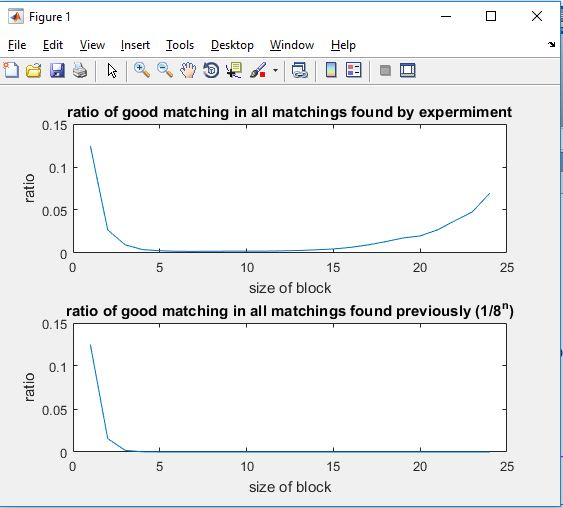
\includegraphics[width=90mm]{ratio.jpg}
So we can see that the ratio follow the $\frac{1}{8^n}$ until blocksize 15, then it goes up again to almost match 1/8 for blocksize 24. With the current algorithm and this size of block the number of iteration would be $8^d$ and as $d = 24$ is really large it's still not effective.\\
Even if the ratio do not behave as previously thought, the complexity stay too high for reasonable blocksize between 8 and 14, and if you go in higher blocksize, the ratio is good but the complexity depends on a ratio power the blocksize, so it will not be good enough to be taken in account.

\subsection{Experiment 3:Blocksize and diffence of block in n ciphers}

\begin{tabular}{|l|c|r|}
  \hline
  blocksize & Probability that 2 blocks are different & \# maximal of ciphers for $\Pr > 0.95$\\
	1 & (0.9367250929) & less than 1\\
	2 & (0.99290120378) & 7\\
	3 & (0.99868328054) & 38\\
	4 & (0.99971599715) & 180\\
	7 & (0.99998010694) & 2578\\
	10 & (0.99999683297) & 16195\\
	12 & (0.99999899833) & 51207\\
	14 & (0.99999959261) & 125907\\
	16 & (0.99999985551) & 354995\\
	\hline
\end{tabular}

Indeed, it's obvious that the bigger the block is, the lower is the chance that you have another one with the same value. For blocksize 1, you cannot hop to have a good probability to get another block different as there are only 26 possibilities. You just have to resolve the following:$Probability^{\#ciphers}>0.95 = n < \frac{\log(0.95}{\log(Probability)}$.
\appendix
\newpage
\section{Algorithm}
You hash a reference text.\\
You take the key matrix that you get from algorithm 1, find plain text in $\mathbb{Z}/2\mathbb{Z}$, and create an array.\\
find the list of all matching: find all pairs $(seg,str)$ such that $seg$ is a segment of plaintext modulo 2 and $str$ $\in hash(seg)$ and save it in a list.\\
\begin{algorithmic}[1]
	\REPEAT
\STATE select d matching form list (you'll get a $d\times d$ key matrix)
\FOR{each of these matchings ($seg_{i}$, $str_{i}$)}
	\STATE extract $block_{i}$ from $seg_{i}$ and $str'_{i}$ from $str_{i}$,
	\STATE then find $ciphertext_{i}$ such that $K^{-1}$ x $ciphertext_{i}$ mod 2 = $block_{i}$
\ENDFOR
\STATE solve $ciphertext_{i} = K * str'_{i}$ for i=1 to d
\STATE compute $K^{-1} * $ciphertext
\UNTIL decryption make sense
\end{algorithmic}
number of iteration is $ \frac{1}{ratio^{nd}} = 8^{nd}$
\\
\\
The following algorithm is to recover the key matrix in $\mathbb{Z}/2\mathbb{Z}$\\
\begin{algorithmic}[1]
\STATE Part1:\\
\REQUIRE{Ciphertext $Y_1,Y_2,...,Y_n$}\\
\ENSURE{K($\bmod 2$)}\\
\FORALL{$\mu$}
	\STATE compute $S_n(\mu) = \sum_{k=1}^{n}{(-1)^{\mu.y} \times n_y}$ where $n_y=\#\{k;Y_k=y\}$
\ENDFOR
\STATE set all $\mu$ to the d values of $\mu$ with largest $S_n(\mu)=bias(\mu.Y)$
\STATE Part2:\\
\FORALL{$(i,i')$}
	\STATE compute $n_{00}(i,i')=\#\{k<n:(\mu_i .Y_k,\mu_i'.Y_{k+1})=(0,0)\}$
\ENDFOR
\STATE set $(i_d,i_1)$ to the first pair with lowest $n_{00}$
\\
\STATE Part3:\\
\FORALL{$t=2$ to $d-1$}
	\FORALL{i $\notin \{i_1,i_2,..,i_{t-1},i_d\}$}
		\STATE compute $n_{00}(i,i{'})=\#\{k:(\mu^{T}_{i_{t-1}}Y_{k},\mu^{T}_{i}Y_{k})=(0,0)\}$\\
	\ENDFOR
	\STATE take i such that $n_{00}$ is minimum and set $i_t=i$\\
\ENDFOR
\STATE set $\mu = (\mu_{i1},\mu_{i1},...,\mu_{id})$ and $K=(\mu^-1)^T$
\STATE output K
\end{algorithmic}
Here to be faster we store $n_y$ in a table and we do a FFT on this table to get $S_n$. With this operation the total complexity drop from $O(d^2 \times 2^d)$ to $O(d \times 2^d)$
But it seems with some other techniques we could do better.


\section{References}

[1] Alina, Matyukhina. \textit{Cryptanalysis of the Hill Cipher}.\\
\\[0pt]
[2] S. Shazaei, S. Ahmadi. \textit{Ciphertext- only attack on} $d \times d$ \textit{Hill in} $O(d13^d)$.\\
\\[0pt]
[3] Akavia, A. \textit{Deterministic Sparse Fourier Approximation via Fooling Arithmectic Progressions}.\\
\\[0pt]
[4] Akavia, A., Goldwasser, S., Safra, S. \textit{Proving Hard-Core Predicates Using List Decoding}.\\
\\[0pt]
[5] Hassanieh, H., Indyk, P., Katabi, D., Price, E. \textit{Nearly optimal sparse Fourier transform}.\\
\\[0pt]
[6] Hassanieh, H., Indyk, P., Katabi, D., Price, E. \textit{Simple and practical algorithm for sparse Fourier transform}.\\
\\[0pt]
[7] Iwen, M.A. \textit{Combinatorial Sublinear-Time Fourier Algorithms}.\\
\\[0pt]
[8] http://www.nymphomath.ch/crypto/stat/anglais.html\\



\end{document}
